\documentclass[tikz,border=3.14mm]{standalone}
\usetikzlibrary{shapes,arrows.meta}
\tikzset{
block/.style={rectangle, draw, text centered, rounded corners},
line/.style={draw, -{Latex[length=2mm]}}
}
\begin{document}
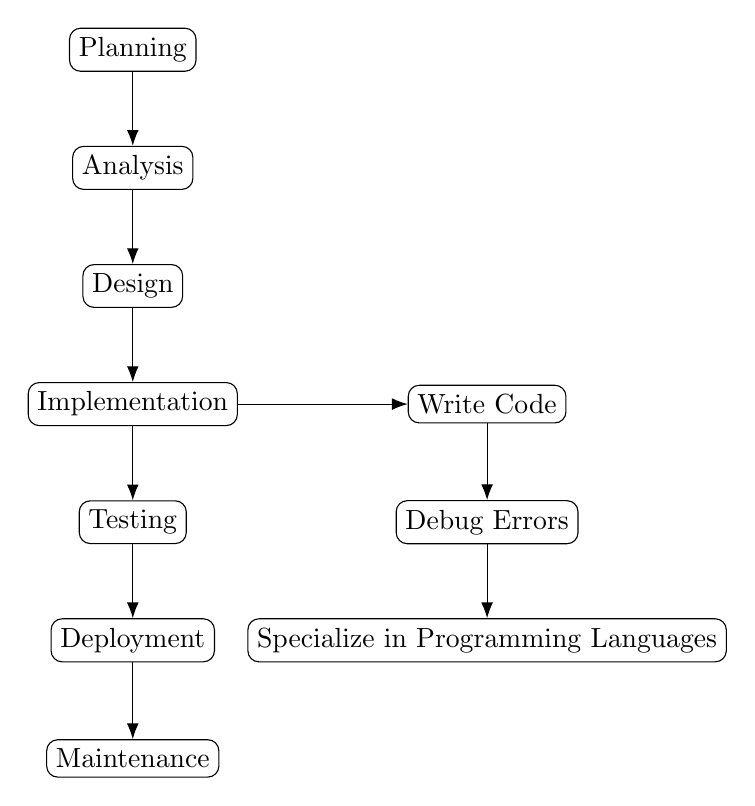
\begin{tikzpicture}[node distance = 1.5cm, auto]
    % Place nodes
    \node [block] (planning) {Planning};
    \node [block, below of=planning] (analysis) {Analysis};
    \node [block, below of=analysis] (design) {Design};
    \node [block, below of=design] (implementation) {Implementation};
    \node [block, right of=implementation, xshift=3cm] (writecode) {Write Code};
    \node [block, below of=writecode] (debug) {Debug Errors};
    \node [block, below of=debug] (specialize) {Specialize in Programming Languages};
    \node [block, below of=implementation] (testing) {Testing};
    \node [block, below of=testing] (deployment) {Deployment};
    \node [block, below of=deployment] (maintenance) {Maintenance};
    % Draw edges
    \path [line] (planning) -- (analysis);
    \path [line] (analysis) -- (design);
    \path [line] (design) -- (implementation);
    \path [line] (implementation) -- (testing);
    \path [line] (testing) -- (deployment);
    \path [line] (deployment) -- (maintenance);
    \path [line] (implementation) -- (writecode);
    \path [line] (writecode) -- (debug);
    \path [line] (debug) -- (specialize);
\end{tikzpicture}
\end{document}